\documentclass[conference]{IEEEtran}
\usepackage{amsmath,amssymb}
\usepackage{graphicx}
\usepackage{booktabs}
\usepackage{siunitx}
\usepackage{cite}
\usepackage[hidelinks]{hyperref}
\graphicspath{{../results/}}
\sisetup{group-digits=false}
\setlength{\textfloatsep}{8pt plus 2pt minus 2pt}
\setlength{\abovedisplayskip}{4pt}\setlength{\belowdisplayskip}{4pt}

\begin{document}
\title{A Nodal Electromagnetic Transient Solver\\With Trapezoidal Companion Models}
\author{\IEEEauthorblockN{Haoran Liu}
\IEEEauthorblockA{CloudDRTS preparation, Phase 2\quad November 2026}}
\maketitle

\begin{abstract}
A small nodal electromagnetic transient (EMT) solver is written in Python with trapezoidal companion models for resistors, inductors and capacitors, ideal voltage sources, switches and the lossless Bergeron line. It is validated against analytic solutions of RC, RL and RLC circuits, a switched RLC circuit and a mismatched transmission line at time steps from \SI{100}{\micro\second} to \SI{5}{\micro\second}. All lumped cases converge with order 2.00, the line is reproduced to round-off, and a second solve at switching instants is shown to be necessary to keep second-order accuracy across events.
\end{abstract}
\begin{IEEEkeywords}
Electromagnetic transients, nodal analysis, trapezoidal rule, Bergeron line model.
\end{IEEEkeywords}

\section{Introduction}
EMT programs solve the network at a fixed time step with each dynamic element replaced by a discrete companion model~\cite{dommel,watson}. This solver is the basis of the partitioning study of Phase~3, which relies on the decoupling property of the Bergeron line. Its accuracy is therefore established here against closed-form solutions before it is used.

\section{Method}
\subsection{Companion models and nodal equations}
Integrating $v=L\,\mathrm{d}i/\mathrm{d}t$ and $i=C\,\mathrm{d}v/\mathrm{d}t$ with the trapezoidal rule over one step $\Delta t$ gives a conductance in parallel with a history current source,
\begin{align}
i_L(t)&=\frac{\Delta t}{2L}\,v_L(t)+\underbrace{i_L(t-\Delta t)+\frac{\Delta t}{2L}\,v_L(t-\Delta t)}_{h_L(t)},\\
i_C(t)&=\frac{2C}{\Delta t}\,v_C(t)\underbrace{-\,i_C(t-\Delta t)-\frac{2C}{\Delta t}\,v_C(t-\Delta t)}_{h_C(t)}.
\end{align}
Each step is then one linear solve
\begin{equation}
G\,v(t)=i_s(t)-B\,h(t)-G_{uk}\,v_k(t),
\end{equation}
where $G$ is the conductance matrix of the unknown nodes, $B$ the incidence of the companion sources, and $v_k$ the prescribed voltages of ideal sources, whose coupling $G_{uk}$ is moved to the right-hand side. A switch adds the conductance $1/R_\mathrm{on}$ when closed.

\subsection{Switching instants}
At a switching instant the step is first computed with the old topology. The same instant is then solved again with the new topology, with capacitor voltages and inductor currents held as constraints (an augmented system with one Lagrange multiplier, the capacitor current, per capacitor), and the histories restart from the new values. Without this second solve the histories carry the pre-switching currents into the next interval, which introduces an $O(\Delta t)$ error at every event.

\subsection{Lossless line}
With currents positive into the line at both ends $k$ and $m$, the Bergeron model~\cite{dommel} is
\begin{equation}
i_k(t)=\frac{v_k(t)}{Z}+h_k(t),\quad h_k(t)=-\frac{2v_m(t-\tau)}{Z}-h_m(t-\tau),
\end{equation}
so that each end is a conductance $1/Z$ with a source that depends only on the other end one travel time $\tau$ earlier. The two ends are decoupled within a step, which allows the network to be split at the line. The travel time is required to be an integer multiple of $\Delta t$; no interpolation is used.

\section{Validation}
\begin{table}[!t]
\caption{Maximum Error Against the Analytic Solutions}
\label{tab:val}
\centering\footnotesize\setlength{\tabcolsep}{3pt}
\begin{tabular}{@{}lccc@{}}
\toprule
Case & \SI{50}{\micro\second} & \SI{5}{\micro\second} & Order\\
\midrule
RC, \SI{10}{\ohm}, \SI{100}{\micro\farad} & \SI{7.7e-5}{V} & \SI{7.7e-7}{V} & 2.00\\
RL, \SI{10}{\ohm}, \SI{10}{\milli\henry} & \SI{7.7e-6}{A} & \SI{7.7e-8}{A} & 2.00\\
RLC, \SI{6}{\ohm}, \SI{10}{\milli\henry}, \SI{10}{\micro\farad} & \SI{8.1e-3}{V} & \SI{8.1e-5}{V} & 2.00\\
RLC, switched shunt & \SI{6.2e-3}{V} & \SI{6.2e-5}{V} & 2.00\\
\quad without second solve & \SI{2.6e-2}{V} & \SI{2.6e-3}{V} & 1.00\\
Line, $Z=\SI{50}{\ohm}$, $\tau=\SI{0.5}{ms}$ & \SI{2.2e-16}{V} & \SI{2.2e-16}{V} & exact\\
\bottomrule
\end{tabular}
\end{table}
\begin{figure}[!t]
\centering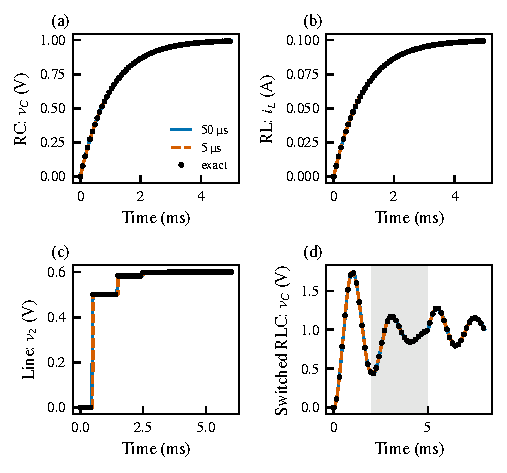
\includegraphics[width=\columnwidth]{phase2_waveforms.pdf}
\caption{Computed responses at \SI{50}{\micro\second} (solid) and \SI{5}{\micro\second} (dashed) against the analytic solutions (dots): (a) RC, (b) RL, (c) receiving-end voltage of the mismatched line, (d) RLC with the shunt closed in the shaded interval.}
\label{fig:wave}
\end{figure}
\begin{figure}[!t]
\centering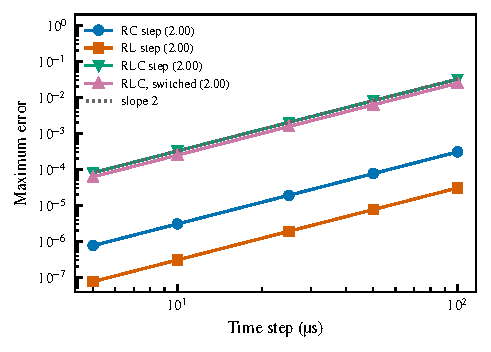
\includegraphics[width=\columnwidth]{phase2_convergence.pdf}
\caption{Maximum error against the time step; fitted orders in brackets.}
\label{fig:conv}
\end{figure}
All cases are driven by a \SI{1}{V} step at $t=0$. The RC, RL and series RLC (underdamped) circuits are compared with their closed-form step responses. In the switched case a \SI{100}{\ohm} resistor is connected across the capacitor of the RLC circuit at \SI{2}{ms} and removed at \SI{5}{ms}; the reference is obtained interval by interval with the matrix exponential. The line case uses a source resistance of \SI{100}{\ohm} and a load of \SI{150}{\ohm}, giving reflection coefficients $1/3$ and $1/2$ and the lattice solution
\begin{equation}
v_2(t)=0.6\bigl(1-6^{-n(t)}\bigr),\qquad n(t)=\Bigl\lfloor\frac{t-\tau}{2\tau}\Bigr\rfloor+1 .
\end{equation}

Table~\ref{tab:val} and Figs.~\ref{fig:wave}--\ref{fig:conv} summarize the results. The orders are fitted over steps of 100, 50, 25, 10 and \SI{5}{\micro\second}. All lumped cases converge with order 2.00, as expected for the trapezoidal rule; reducing the step from 50 to \SI{5}{\micro\second} lowers the error by a factor of 100. In the switched case, capacitor voltage and inductor current are exactly continuous across both events. If the second solve at the switching instants is omitted, the same case converges only with order 1.00, and the error at \SI{5}{\micro\second} is 40 times larger. The line is reproduced to round-off at both steps, because the Bergeron model of a lossless line has no truncation error when $\tau$ is a multiple of $\Delta t$; any line error in Phase~3 is therefore caused by the interface and not by the line model. Finally, for an undamped LC circuit the stored energy stays constant within a relative $6\times10^{-13}$ over 4000 steps, a known property of the trapezoidal rule.

\section{Conclusion}
The solver is second-order accurate for lumped elements, including switching events when the switching instant is solved a second time, and exact for the lossless line. Its limits are a fixed step, switching only at step boundaries, travel times rounded to whole steps, and single-phase lossless lines. Interruption of an inductor current is not supported, so the numerical oscillations of the trapezoidal rule in that situation are not addressed.

\begin{thebibliography}{1}
\bibitem{dommel} H.~W. Dommel, ``Digital computer solution of electromagnetic transients in single- and multiphase networks,'' \emph{IEEE Trans. Power App. Syst.}, vol.~PAS-88, no.~4, pp.~388--399, Apr. 1969.
\bibitem{watson} N.~Watson and J.~Arrillaga, \emph{Power Systems Electromagnetic Transients Simulation}, 2nd~ed. London: IET, 2018.
\end{thebibliography}
\end{document}
